\documentclass{ba-kecs}
\usepackage{graphicx,, url}
\usepackage[numbers]{natbib}
\usepackage{amssymb,amsmath}

\title{Turtlebot SLAM }

\author{Maurice Hermans, Lukas Kang, Michael Norget, Thomas Nowicki, Oliver Trinnes}

\begin{document}

\maketitle

\begin{abstract}
This article accompanies the research project "TurtleBot SLAM" from the Master "Artificial Intelligence" of Maastricht University.
\end{abstract}

\section{Introduction}
\label{sec:intro}
Nowadays mobile robots are able to assist humans in a diverse set of problems. Transportation, search, rescue and automated vacuum cleaning are examples from different fields. Typically, mobile robots can move through an environment using legs or wheels. In addition they are able to gather information about their environment using sensors. Some even have devices similar to the human arm or hand which allows them to interact with the environment. The vaccuum cleaning robot presented in Figure \ref{fig:vacuum_cleaner} is an example of a robot which has whells to move around. Furthermore it is equipped with a set of sensors. These sensors provide data about the location of obstacles as well as, for example, gaps in the floor the robot is moving on. To efficiently perform this task robots needs a map of its environment. For some tasks map data is available for the robot from the beginning. Provided a map the robot can locate itself using the incoming sensor data. For tasks in unknown environments, however, the robot must rely on internal sensors and make its own map of the environment.

The acquisition of these maps has been a major research focus in the robotics community \cite{Grisetti} [\textbf{MORE SOURCES}]. Building or learning these maps under position uncertainty provided only sensor measurements is often referred to as the Simultaneous Localization And Mapping (SLAM) problem. A large variety of solutions is available to the SLAM problem, these approaches can be classified as either filtering or smoothing [\textbf{SOURCE}].

Filtering approaches model the problem as a so called ``on-line" state estimation problem. The state of such a system consists of the current robot position and the map. New measurements augment and refine the estimate as they become available. Due to their incremental nature these filtering approaches are commonly referred to as on-line SLAM methods. The other type of approach estimates the full trajectory from the full set of measurements. These approaches address the so called full SLAM problem and they typically rely on least-square error minimization techniques [\textbf{SOURCE}].

An intuitive way to formulate the SLAM problem is to consider it as a pose graph optimization problem. The nodes of the graph represent robot poses or landmarks. The edges encode sensor measurements that constraint the connected poses. Once such a graph is constructed the graph-based SLAM method tries to find a configuration of the nodes that is maximally consistent with the contraints contained in the edges. (\textbf{ABSTRACT GRAPH PICTURE HERE})

The rest of this paper is structured as follows. Section \ref{sec:sota} provides the reader with the necessary background information on the topic. Section \ref{sec:impl} is about the implementation details of the methods used. Section \ref{sec:exp} explains the experiments ran to validate and benchmark the implemented methods and also evaluate the obtained results. Section \ref{sec:disc} discusses the acquired results of the experiments and proposes further research based on those. And the last section wraps up the paper with the conclusions of this research.

\begin{figure}[htp]
	\centering
		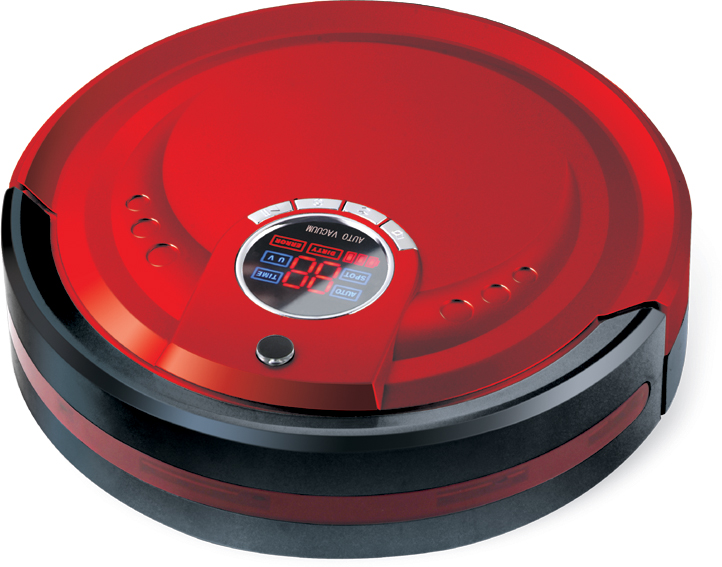
\includegraphics[width=0.50\textwidth]{figures/vacuum_cleaner.jpg}
	\caption{Automated vacuum cleaner}
	\label{fig:vacuum_cleaner}
\end{figure}

\subsection{Problem Statement}
\label{sec:problem}
This paper accompanies a university group project. The project assignment is to implement both a graph-based SLAM algorithm and an autonomous exploration strategy. The hardware to be used is a mobile robot called TurtleBot. Thus the final product should allow the robot to autonomously navigate through an unknown environment and simultaneously build a map of it using a graph-based SLAM algorithm. Information about SLAM methods, autonomous exploration and the TurtleBot are given in Section \ref{sec:sota}.  

\section{State of the art}
This section presents the state of the art of the hardware, software, and methods used for this project. Subsection \ref{subsec:ros} gives an outline about the operating system in which the product is implemented. Next, Subsection \ref{subsec:turtle} is about the TurtleBot. At last, autonomous exploration (Subsection \ref{subsec:sotaExplore}) and SLAM (Subsection \ref{subsec:sotaSlam}) 
\label{sec:sota} are defined and explained.
\subsection{ROS}
\label{subsec:ros}
The Robot Operating System (ROS) \cite{Quigley} is the environment used throughout the development of all product components for this project. As described by Quigley et al., writing software for robots is difficult since there is a huge variety of possible hardware setups. This also makes code reuse non-trivial. An additional problem is the amount of code needed to acttually ``run" something on a robot. A deep stack including driver-level software, perception modules and, for example, abstract reasoning systems is required before the actual problem can be attacked. Since the necessary expertise and effort is beyond capabilities of most single researchers, an environment that features this functionality is required to achieve anything similar to the problem specified in Subsection \ref{sec:problem}.

To deal with the above mentioned problems robotics researchers have created a wide variety of frameworks. Many robotic software systems are currently used by researchers and industry \cite{Kramer}. Each of these frameworks is designed for one specific purpose. Generally, none of these systems is directly applicable to a problem it was not designed for in the first place.

The ROS framework used in this paper is the product of trade-offs and prioritizations. The emphasis of this framework lies on large-scale integrative robotics research, making it useful in a wide variety of situations. The difference between ROS and the above mentioned frameworks, is ROS' applicability to a wide range of hardware setups.  It provides several so called stacks. Each is an assembly of code made to solve one specific problem. To run a stack or your own code on any robot it is necessary to configure the robot and the ROS framework in a way that they can communicate with each other. For most robots the configuration is straight forward thanks to the online documentation of ROS \citep{Roswiki}.  An example for a stack is the multi-robot simulation environment ``Stage". It is explained in the following paragraph.

\subsubsection{Simulation}
During the development process of a system running on a robot one curcial part is testing. A ROS stack called Stage enables the developers to test code on a simulated robot. Stage allows the simulated robot to move around in virtual environments. It visualizes sensor data and other robot data when required. The user can load her own maps into stage and specify the kind of noise to be applied to measurements. A second important stack needed especially for validation is RViz. It visualizes all requested data. In Figure \ref{fig:stage_and_rviz} Stage and RViz are presented next to each other. While Stage (Left) shows the real map, RViz (Right) presents the map data as seen by the robot.

\subsection{TurtleBot}
 \label{subsec:turtle}

The product of this project is designed to run on a robot called TurtleBot(Figure \ref{fig:turtlebot}). The TurtleBot is a low-cost, customizable, personal robot kit (\textbf{PARAPHRASE?}).The base of the TurtleBot is an iRobot Create (A). It holds a battery pack and 150 degrees/second Single Axis Gyro. The model shown in Figure \ref{fig:turtlebot} uses a Microsoft Kinect sensor (B), the one used in this paper uses a laser range sensor, and a laptop (C) to run all the processes. The robot can also be customized using the mounting hardware (D). The robot runs on an open-source SDK based on ROS which integrates all the software needed to get the TurtleBot running. Already included are some advanced capabilities like mapping and navigation.
\begin{figure}[h]
	\centering
		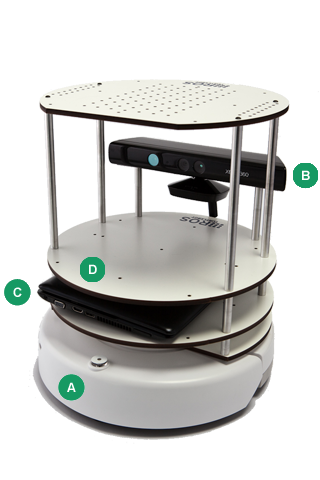
\includegraphics[width=0.50\textwidth]{figures/turtlebot.png}
	\caption{A TurtleBot}
	\label{fig:turtlebot}
\end{figure}

\subsection{Exploration}
\label{subsec:sotaExplore}
Usually robots localize themselves and navigate through environments using a map which is provided by an external source. In this case navigating from one location to another is an easy problem. If, however, the robot does not have access to a map, navigating through an environment is problematic. The problem treated in this paper (Subsection \ref{sec:problem}) assumes an unknown environment and, hence, no map. The robot needs to be able to explore its environment without any knowledge about it. It needs to rely on the incoming laser and odometry data only. In addition to the creation of the map and the localization of itself (the SLAM problem) the robot needs to explore the environment as efficient as possible. We define a good exploration strategy as one that generates an accurate map in the shortest amount of time.

Ideally the robot updates its internal map of the environment constantly while moving. One idea to efficiently explore the environment is to move to locations which maximize the robots information gain. This target location needs to be extracted from the limited information the robot has collected with its sensors.
To achieve this the robot makes use of the idea of frontier-based exploration, first introduced by Yamauchi \cite{Yamauchi} in 1998 (\textbf{REALLY?}). Frontiers are defined to be the boundaries between free and unexplored space. Intuitively, when a robot moves to a frontier it is likely that it makes measurements in previously unexplored space. Assuming that the new data is immediately added to its map, the explored region grows once the robot reaches a frontier. Moreover an extended map results in new frontiers. By constantly moving to frontiers the robot expands its knowledge about the environment.

\subsection{SLAM}
\label{subsec:sotaSlam}
As mentioned in Section \ref{sec:intro} Simultaneous Localization And Mapping (SLAM) is the process of building a map based on sensor data while simultaneously localizing yourself in an unknown environment.

SLAM is a problem because, generally, localization requires a map and mapping requires the loacation of a device or a robot that wants to create a map. There are quite a few approaches that successfully solve the SLAM problem. Mostly, filtering techniques like Kalman filters Particle filters and Information filters are used to estimate the state of the system. FastSlam \citep{Montemerlo02} is an example of a SLAM implementation using a particle filter to approximate the robots trajecotry and positions of landmarks on the map. 

Conversely, the smoothing approaches keep using all measurements to estimate the entire trajectory the robot has traveled.
\textbf{TODO: CONNECTION}
\subsubsection{GraphSLAM}
An intuitive way to formulate the SLAM problem is to view it as a pose graph optimization problem. A graph will be constructed where the nodes represent robot poses or landmarks and where edges correspond to measurements that constraint the connecting nodes. Note that constraints can be contradictory because of the noise on the measurements. Once a graph is constructed the algorithm will try to find a configuration of the nodes that is maximally consistent with the measurements.

\section{Implementation}
\label{sec:impl}

The implementation used for this paper is written on a Linux operating system. Programming has been done using ROS and the object oriented programming language C++. The installation process for ROS, as done in this paper, can be reviewed on Maastricht's swarmlab homepage \cite{swarmlab}.
 For the coding part there exist two main packages, one of which includes the exploration and the other one the mapping part of the SLAM problem. To enable the robot with exploration capabilities, the ROS internal navigation stack for the TurtleBot has been used, making movement possible, by sending a designated goal to the robot.

\subsection{Wavefront frontier detection}

As a part of the assignment the robot has to drive autonomously through an unknown map. This feature is implemented using Wavefront frontier detection (WFD).

WFD is using frontiers for its exploration purposes. Creation of frontiers requires the robot to know about the current environment in form of a map. In this example an Occupancy grid is used \ref{sec:mapping}. The general algorithm is then applied to acquire four different data structures that store map and frontier information. These four data structures are :
\newline
1. Map-Open-List
\newline
2. Map-Close-List
\newline
3. Frontier-Open-List
\newline
4. Frontier-Close-List 
\newline
 
To understand the need of these four structures it is necessary to know that WFD is using a breadth first search (BFS), starting at the current robot position that has to be passed into the algorithm. WFD also requires a current map representation, which is acquired by the mapping package in this program.
Upon launching the algorithm it first searches for unoccupied space around the current robot location, which is then saved into the Map-Open-List. 
Frontiers are found by making use of the occupancy grid's structure. A criterion for a point to be a frontier is that it has to have unknown space and known unoccupied space around it. If a frontier point is found a new BFS is performed, to extract all adjacent frontier points and connect them to one consistent frontier into the Frontier-Open-List. The benefit of using WFD is that by maintaining these lists, rescans only need to incorporate points that have not been scanned yet, as the algorithm saves detected open space and frontiers into its adjacent close lists, if a point is rescanned. For up following scans these points are no longer considered and by that the algorithm does not need to be rerun all over again.
 
 Detecting frontiers and navigating towards them directly is not possible due to ROS's navigation stack. Instead of sending the robot the goal to a frontier point, an algorithm has to be performed to find a point next to the frontier cell with as much free space around it as possible. For detection purposes an evaluation function for the frontiers has been written, which incorporates three features that are used to send a goal to the robot's navigation stack. The three features are :
 \newline
 1. distance of frontier to the robot location
  \newline
 2. number of obstacles around the designated frontier
  \newline
 3. - ?
  \newline
  
  The features are added up and the sum is used for the final goal for the navigation stack. By applying these three features the robot can always access the next point and is by that able to drive throughout the whole map and perform the algorithm and exploration perfectly.
\subsection{GraphSLAM}
Two different approaches of graph-based SLAM are implemented for this project. They differ in complexity and thereby applicability to the problem. Both algorithms create an occupancy grid map. 

First, an algorithm as suggested by \citep{Grisetti} is implemented. Here the graph consists of nodes representing positions along the robot trajectory. Odometry and sensor measurements are incorporated into the constraints contained in the edges. Again, an edge connects two adjacent poses of the robot. This graph-based SLAM approach optimizes the pose graph according to the constraints. This ``optimized" trajectory then determines the positions of obstacles on the map by refining the laser scan data according to the poses they were obtained at. Each edge thus is labelled with the spatial difference between two poses \(x_i\) and \(x_j\). Let this error be denoted by \(e_{ij}(x_i, x_j)\). This graph-based SLAM approach calculates the most likely path as follows:
First it calculates the Jacobians \(A\) and \(B\) of every two estimated positions connected by an edge.
\begin{equation}
\label{eq:jacobi_a}
	A_{ij} = \frac{\partial e_{ij}(x)}{\partial x_i}\uplus
\end{equation}
\begin{equation}
\label{eq:jacobi_b}
	B_{ij} = \frac{\partial e_{ij}(x)}{\partial x_j}
\end{equation}
Note that in Equations \ref{eq:jacobi_a} and \ref{eq:jacobi_b} the x represents the current guess of the concerning robot position. These Jacobians are then added to an information matrix \(H\) (see Equation \ref{eq:H}).
\begin{equation}
\label{eq:H}
\begin{aligned}
	H_{[ii]} += A^{T}_{ij} \Omega_{ij} A_{ij} \\
	H_{[ij]} += A^{T}_{ij} \Omega_{ij} B_{ij} \\
	H_{[ji]} += B^{T}_{ij} \Omega_{ij} A_{ij} \\
	H_{[jj]} += B^{T}_{ij} \Omega_{ij} B_{ij} \\
\end{aligned}
\end{equation}
Furthermore a coefficient vector \(b\) is always updated as shown in Equation \ref{eq:b}. This vector in combination with the \(H\) matrix form a set of linear constraints.
\begin{equation}
\label{eq:b}
\begin{aligned}
	b_{[i]} += A^{T}_{ij} \Omega_{ij} e_{ij} \\
	b_{[j]} += B^{T}_{ij} \Omega_{ij} e_{ij} 
\end{aligned}
\end{equation}
Optimizing the vector \(x = (x_1, ..., x_n)^T \) according to the constraints specified in \(H\) and \(b\) is the core of this approach. This step is performed using sparse Cholesky factorization. 
A new node is added to the graph once the robot moved 0.5 meters. The algorithm optimizes the trajectory like explained when a new node is added. In one special case the algorithm adds and edge connecting to non-adjacent nodes to the graph. This happens when the distance between the two connected robot positions is smaller than a margin. In fact, this special case enables the algorithm to create loops in the graph and more accurately estimate the robots trajectory and the map. This procedure is referred to as ``loop closing". 
\\
\\
The second implementation is based on \cite{Thrun}. It creates nodes for each odometry measurement of the robot as well as for each feature in the map spotted by the laser sensor. Each occupancy grid cell containing an obstacle is considered a map feature. Edges are labelled with spatial constraints of the two nodes they are connecting. The output of this implementation is a vector containing the positions of the land marks as well as the trajectory of the robot. Here the constraints labelling the edges ar created using Jacobians similar to the previous approach. The major difference lies in the node creation. Here nodes are added for landmarks while the previous implementation considered the robots' trajectory only. Since no obstacle in the final occupancy grid must be missed all obstacle points are treated as landmarks for this implementation. 
\subsubsection{Scan matching}

The scan matcher, used by this program, is necessary to acquire an optimized movement vector between two robot positions, which is needed by the GraphSLAM algorithm. The programming of the scan matcher used requires two steps. For the first step the two scans are matched together by making use of raw odometry data, retrieved by the robot's motion sensor. The improvement done by the scan matcher is then to run an iteration of the iterative closest point algorithm (ICP), to incorporate its perception with the movement. 

The general procedure of the algorithm is to first find corresponding neighbors. These are found by using the nearest neighbor search, through which adjacent points are found by calculating two points from different sets according to their euclidean distance to one another. Points in this implementation can have multiple correspondences to neighbors. To avoid incorporating outlying points, a fixed distance has been set. Outliers would otherwise impact further calculations negatively.
The next step in the process is to calculate center points for both clouds, which are needed to normalize them in respect ot each other. After performing the calculation the center points for each cloud are subtracted from every point belonging to that cloud. The calculated points are then added to two separate matrices, both representing one point cloud as a $2xn$ Matrix, where n is the number of neighbor pairs. The first cloud's matrix is then multiplied by the transposition of the second cloud matrix, so that a new matrix is created for which we calculate the Singular Value Decomposition (SVD) values to retrieve a rotational matrix, responsible for rotating the second point cloud to the first one. The next step is to translate the second point cloud to the first one with the use of a translation vector. Both rotation matrix and translation vector are then passed to a matrix containing both of them as well as a third line with the values $0 0 1$, for symmetry purposes. That matrix is then used to adjust the second point cloud to the first one. It is also used to correct the robot position.

\subsection{Mapping}\label{sec:mapping}

For Mapping purposes an Occupancy grid is created on which information about obstacles, free/- and unknown space is saved. Using ROS's visualization program, RVIZ, the map can be visualized entirely.

The occupancy grid is a structure that can be represented by a single dimensional array. Its size is responsible for the size of the grid and is often problem specific, especially for the purpose of Slam. Making the grid too large can lead to performance problems and by that the grid's size gets to be a tunable parameter that has to be chosen carefully for each problem, although making the grid large prevents the robot from going ``out of space''.
 This program converts the array into a two dimensional representation, so that navigating to either side gets more intuitive. Each value of the array is an integer and represents the current status of the cell. The value ranges for ROS's occupancy grid lie between $-1$ and $100$ \cite{occupancy}. Each value has its own meaning :

\begin{description}
\item{$-1$} : unknown space, not yet covered by robot's perception sensors
\item{$ 0$} : known free space, robot can drive on it safely
\item{$1-100$} : probability of being an obstacle, $1$ being a low probability and $100$ being a definite obstacle
\end{description}

\begin{figure}[htbp]
	\centering
		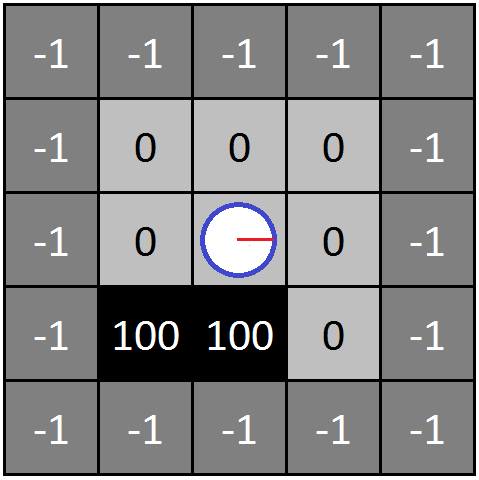
\includegraphics[width=0.50\textwidth,height = 44mm]{figures/Occup.png}
	\caption{Occupancy Grid visualized}
	\label{fig:Occupancy}
\end{figure}

Fig.\ref{fig:Occupancy} shows these three occurrences visualized, with a robot in the middle performing a sample scan of its environment.
The occupancy grid is using laser scan data for this implementation. Each laser scan has information about whether an obstacle has been detected, or whether the maximum range of the scan has been reached. The scan is then transformed into a point cloud to extract its coordinate information and by that, obstacles can be found.

Free space is being incorporated into the map by filling the occupancy grid between a detected obstacle, or detected maximum range point and the current robot position with $0$ values. This is achieved with the help of a linear function. If a point is not the scanner's maximum range away, the point is saved as an obstacle with value $100$.

As time progresses and the robot explores more of its environment the map is constantly updated. This is programmed by saving laser scans for every pose of the robot, which, when traveling for a distance of $0.5$ meters is added and by that the occupancy grid is updated. Upon a loop closure the occupancy grid is optimized with its information about obstacles and free spaces.

\section{Experiments and Results}
\label{sec:exp}
This section demonstrates the results of the Turtlebot SLAM implementation as described in section \ref{sec:impl}. Several outputs of the visualization tool RViz are presented and discussed. Comparisons are drawn between different variations of the implementation and the performance of the program is evaluated.

\subsection{Visualization}
When running the program via the launch file, RViz and Stage are automatically started. Stage shows the robot in its actual position on an accurate test map (see figure \ref{fig:stage_and_rviz} left). RViz shows the current belief of the robot about its environment, position and trajectory (see figure \ref{fig:stage_and_rviz} right).

The components of the pose graph and the environment are highlighted by the following labels:

\begin{description}
\item[green dots: ]past positions of the robot, saved as nodes of the pose graph
\item[red arrows: ]past orientations of the robot, included in the nodes of the pose graph
\item[blue lines: ]measurement constraints between the connected poses
\item[yellow dots: ]frontier points detected by the wavefront frontier detection algorithm
\item[orange dot: ] next navigation goal
\item[black area: ] detected obstacles
\item[light gray area: ] detected free space
\item[dark gray area: ] unexplored space
\end{description}

\begin{figure}[htbp]
	\centering
		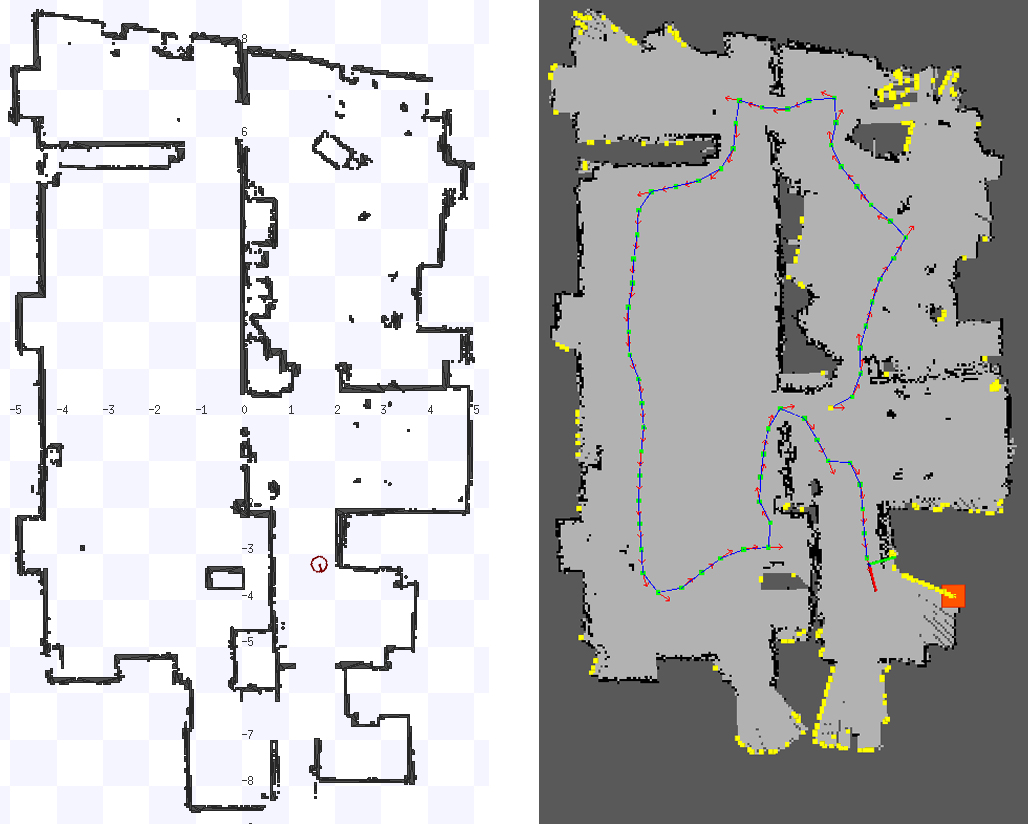
\includegraphics[width=0.50\textwidth]{figures/Stage_and_rviz.jpg}
	\caption{Robot and environment visualization with Stage (left) and RViz (right)}
	\label{fig:stage_and_rviz}
\end{figure}

\subsection{Loop closing effect}
One of the core properties of the Graph SLAM algorithm is the correction of the pose graph and the map whenever a loop closing is detected. This means that when the robot has been exploring an unknown area and then reenters an explored area, the transformation between the current pose and the past re-detected pose gives essential information on the complete pose graph, correcting the current belief about the environment and position.

The effect of loop closing detection is illustrated in figure \ref{fig:loop_closing_comparison}. The transparent red lines indicate the accurate map, while the underlying black areas indicate the belief of the robot about the obstacles of the environment.

The left part of figure \ref{fig:loop_closing_comparison} shows the explored map when walking an eight-shaped path through the map without applying loop detection. It can be seen that the belief about the map differs from the actual map in many areas, especially in the lower half of the map because this half has been explored last, exposing it to most of the measurement uncertainties.

The right part of figure \ref{fig:loop_closing_comparison} depicts the exploration when walking the same path as before but applying loop closing. This results in a pose graph with 7 more constrains, providing more information for correcting the poses and corresponding measurements. One can now see that the lower half of the belief about the map is much more accurate since the area in the center has been re-detected by the algorithm.

\begin{figure}[htbp]
	\centering
		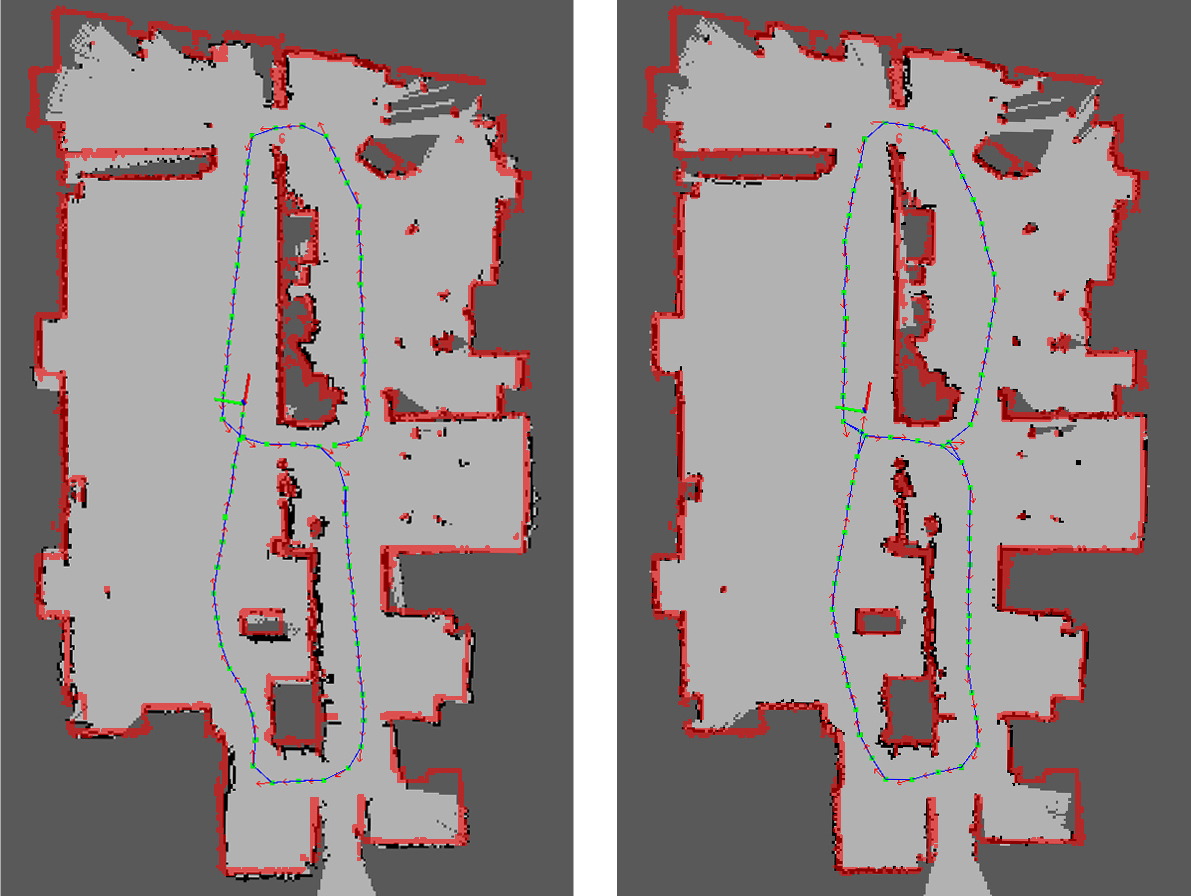
\includegraphics[width=0.50\textwidth]{figures/Loop_closing_compared.jpg}
	\caption{Observed environment without (left) and with (right) loop closing of the pose graph}
	\label{fig:loop_closing_comparison}
\end{figure}

\subsection{Navigation evaluation}
An important aspect which has a high impact on the exploration behavior of the robot is the strategy by which the next navigation goal is determined. When facing the decision for the next goal, the given information are the detected frontiers, which can be spread all over the current map. The most obvious first implementation idea was to select the frontier which lies closest to the robot as the next navigation goal. This is definitely desirable because the robot can then explore this closest point very quickly and find out about the next frontiers.

Figure \ref{fig:navigation_comparison}(a) shows the resulting exploration path of the robot and the explored map after 300 seconds when applying this simple strategy. 10 nodes and 14 constraints have been created in the pose graph during this time which is very little information. Also the nodes are limited a small area of the map. This little degree of exploration is due to the fact that when only considering the closest frontier point there is a high risk that points are selected which are very close to obstacles. When the navigation algorithm tries to find a way to this point, it is inflating the obstacles first, making very close points unreachable. After a point has been discovered to be unreachable, the next closest point to the robot is chosen, which will likely be unreachable as well.

So it can be concluded that the number of close obstacles have to be taken into account in order to select reachable points as next goals. In the upcoming strategy, the sum of obstacles within a radius of 50 grid cells is added to the distance to the robot for every frontier point. The point with the smallest sum is then selected as the next goal. The application of this strategy is shown in figure \ref{fig:navigation_comparison}(b). The robot managed to explore the map within 300 seconds, creating a pose graph with 104 nodes and 150 constraints. However, one can see that the robot did not take a very exploration-efficient route through the map. There are a lot of unreasonable turns in areas that are already explored, while unexplored areas get left out for the time being.

Another aspect is to be added to the evaluation of every frontier point. That is the distance between the currently evaluated frontier point and the previous navigation goal. When this distance is minimized additionally to the distance to the robot and the number of close obstacles, the algorithm will select the next goals in a chain-like fashion, creating a rather intuitive exploration path through the map (figure \ref{fig:navigation_comparison}(c)). The robot was able to explore the map within only 150 seconds, creating a much smaller pose graph of 64 nodes and 66 constraints. This evaluation feature has been given a weight factor of 5 to increase the effect on the goal selection.

\begin{figure}[htbp]
	\centering
		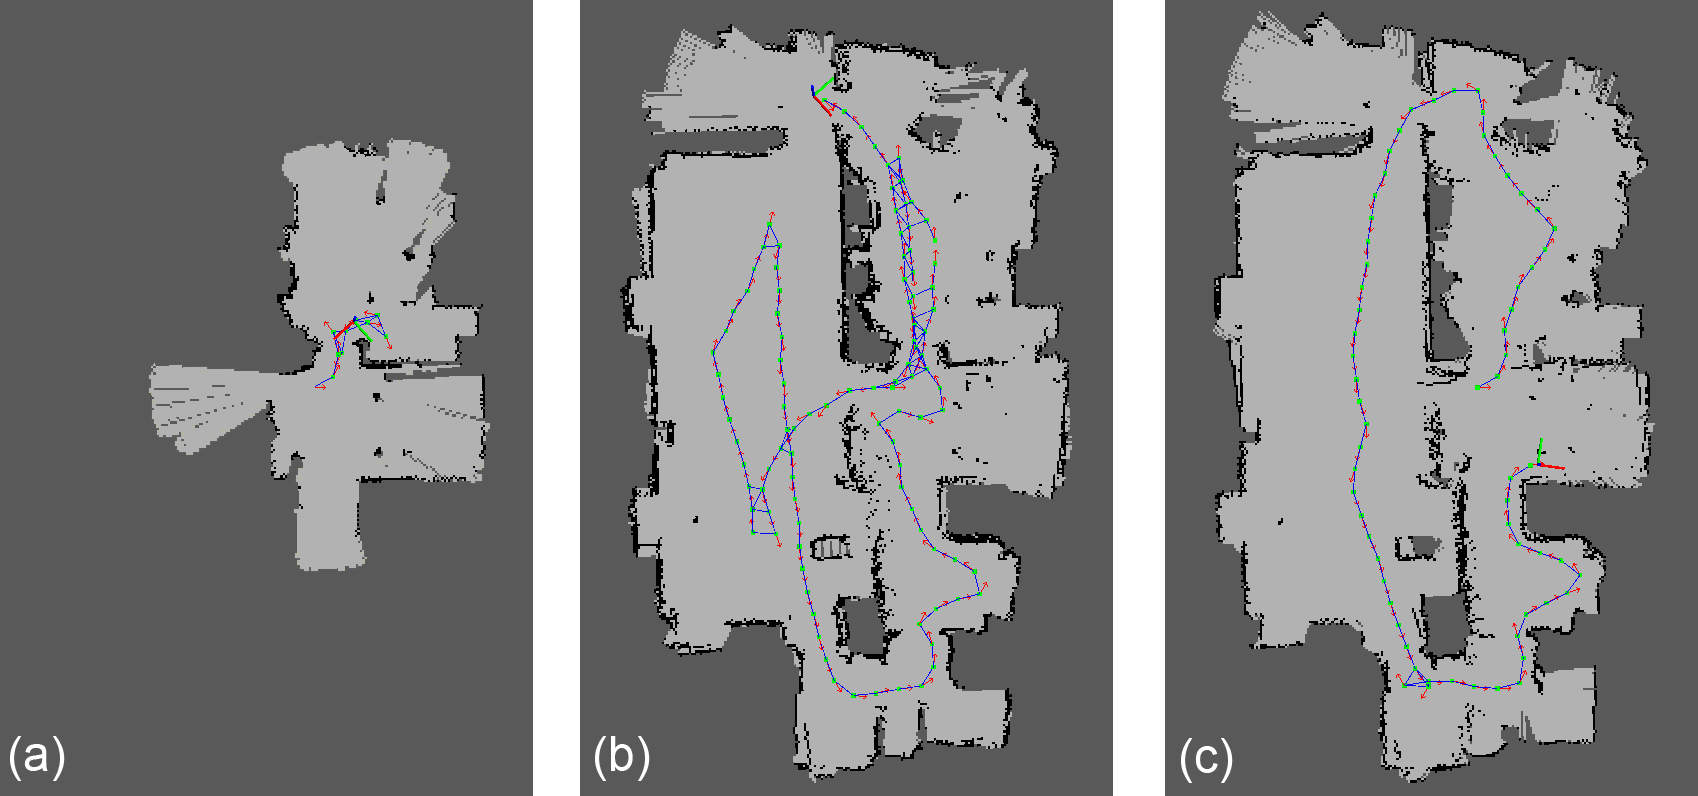
\includegraphics[width=0.50\textwidth]{figures/Navigation_comparison.jpg}
	\caption{Resulting robot trajectory when applying different strategies for selecting the next navigation goal}
	\label{fig:navigation_comparison}
\end{figure}

\subsection{Runtime}

\section{Discussion}
\label{sec:disc}
The Wavefront Frontier detection algorithm \citep{Keidar} succeeds in finding frontiers in a fast and accurate manner.

Implementing the algorithm suggested in \citep{Grisetti} turned out to be well suited for attacking the problem statement of this project. The maps created by this algorithm look accurate. Specifically the margin between the output map and the real map is negligible (FIGURE???). Maps are created in real time and loop closures are added when needed. In fact, the algorithm keeps updating the map with no noticable delay while the robot drives around steering to new goals selected by the WFD algorithm and navigated by ROS' move\_base package.

The second graph-based SLAM implementation \cite{Thrun} clearly is not suited for robots equipped with laser scanners only. Extensive feature extraction methods are required to create occupancy grid maps with the used TurtleBot. Furthermore the algorithm is expected to work best with a robot which is able to detect distinct landmarks as well as a simple environment. A number of unique landmarks can then serve as orientation points to build the map. Additionally the algorithm is able to assess map and trajectory more quickly if there are fewer nodes and constraints in the graph.

\subsubsection{Future research}

\section{Conclusion}
\label{sec:conc}
\bibliography{references}
\nocite{*}
\onecolumn
\appendix

\end{document}
